\subsection{Pose Detection Testing}
\label{subsec:posedetectiontesting}

\begin{figure} [ht]
  \centering
  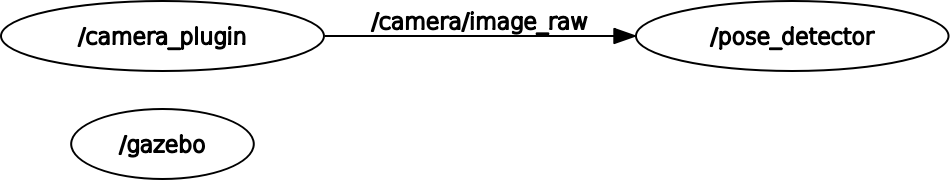
\includegraphics[width=0.45\textwidth]{figures/rosgraph/pose-detection.png}
  \IfLanguageName{english}{
    \caption{Node scheme of the pose detection testing.}
  }{
    \caption{Skema \emph{node} dari pengujian deteksi pose.}
  }
  \label{fig:rosgraphposedetection}
\end{figure}


Pose detection testing is done in the simulation with purpose to test the user model ability in simulating the real user.
In this test,
  \lstinline{pose_detector} node will be run to do a computer vision process in detecting user's pose.
As shown in the figure \ref{fig:rosgraphposedetection},
  \lstinline{pose_detector} node will be connected to the \lstinline{camera_plugin} node that will send user image data which will then be processed by the \lstinline{pose detector} node to produce the detected pose.

\begin{figure} [ht]
  \centering
  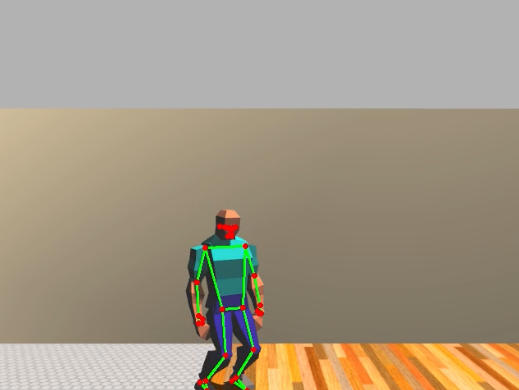
\includegraphics[width=0.4\textwidth]{figures/pose-detection.png}
  \IfLanguageName{english}{
    \caption{User pose detection results.}
  }{
    \caption{Hasil deteksi pose pengguna.}
  }
  \label{fig:posedetection}
\end{figure}


The result,
  as shown in the figure \ref{fig:posedetection},
  from the received image,
  \lstinline{pose_detector} node will detect the user's pose and display the result as lines and dots on the received image.
Besides that,
  the pose detection process could also display the corresponded result when the user's posture is changed from standing to sitting as in the result of figure \ref{fig:posedetection}.
